% ============================================
% CHƯƠNG 3: THIẾT KẾ ỨNG DỤNG
% ============================================

\section{Thiết kế ứng dụng}

% ------------------------------------------
\subsection{Thiết kế cơ sở dữ liệu}

Mặc dù dự án hiện tại sử dụng dữ liệu mock, thiết kế database được xây dựng với tầm nhìn mở rộng trong tương lai.

\textbf{Sơ đồ các entities chính:}

\begin{table}[H]
\centering
\begin{tabular}{|l|l|l|}
\hline
\textbf{Tên trường} & \textbf{Kiểu dữ liệu} & \textbf{Mô tả} \\
\hline
id & INT (PK) & Khóa chính, auto increment \\
username & VARCHAR(50) & Tên đăng nhập \\
email & VARCHAR(100) & Email người dùng \\
password & VARCHAR(255) & Mật khẩu đã hash \\
fullname & VARCHAR(100) & Họ tên đầy đủ \\
phone & VARCHAR(15) & Số điện thoại \\
address & TEXT & Địa chỉ giao hàng \\
role & ENUM & 'customer', 'admin' \\
created\_at & DATETIME & Thời gian tạo tài khoản \\
\hline
\end{tabular}
\caption{Bảng Users - Quản lý người dùng}
\label{tab:users}
\end{table}

\begin{table}[H]
\centering
\begin{tabular}{|l|l|l|}
\hline
\textbf{Tên trường} & \textbf{Kiểu dữ liệu} & \textbf{Mô tả} \\
\hline
id & INT (PK) & Khóa chính \\
name & VARCHAR(200) & Tên sản phẩm \\
slug & VARCHAR(200) & URL-friendly name \\
description & TEXT & Mô tả chi tiết \\
price & DECIMAL(10,2) & Giá bán \\
original\_price & DECIMAL(10,2) & Giá gốc \\
image & VARCHAR(255) & Đường dẫn hình ảnh \\
category\_id & INT (FK) & Liên kết bảng categories \\
author & VARCHAR(100) & Tác giả sách \\
stock & INT & Số lượng tồn kho \\
\hline
\end{tabular}
\caption{Bảng Products - Quản lý sản phẩm}
\label{tab:products}
\end{table}

\begin{table}[H]
\centering
\begin{tabular}{|l|l|l|}
\hline
\textbf{Tên trường} & \textbf{Kiểu dữ liệu} & \textbf{Mô tả} \\
\hline
id & INT (PK) & Khóa chính \\
user\_id & INT (FK) & Liên kết bảng users \\
total & DECIMAL(12,2) & Tổng tiền đơn hàng \\
status & ENUM & 'processing', 'shipping', 'completed', 'cancelled' \\
shipping\_address & TEXT & Địa chỉ giao hàng \\
created\_at & DATETIME & Thời gian đặt hàng \\
\hline
\end{tabular}
\caption{Bảng Orders - Quản lý đơn hàng}
\label{tab:orders}
\end{table}

% ------------------------------------------
\subsection{Kiến trúc MVC tự xây dựng}

Dự án áp dụng mô hình MVC (Model-View-Controller) được xây dựng hoàn toàn từ đầu, không sử dụng framework có sẵn như Laravel hay Symfony. Điều này giúp hiểu sâu về cách thức hoạt động của pattern MVC.

\subsubsection{Luồng hoạt động MVC}

\begin{figure}[H]
\centering
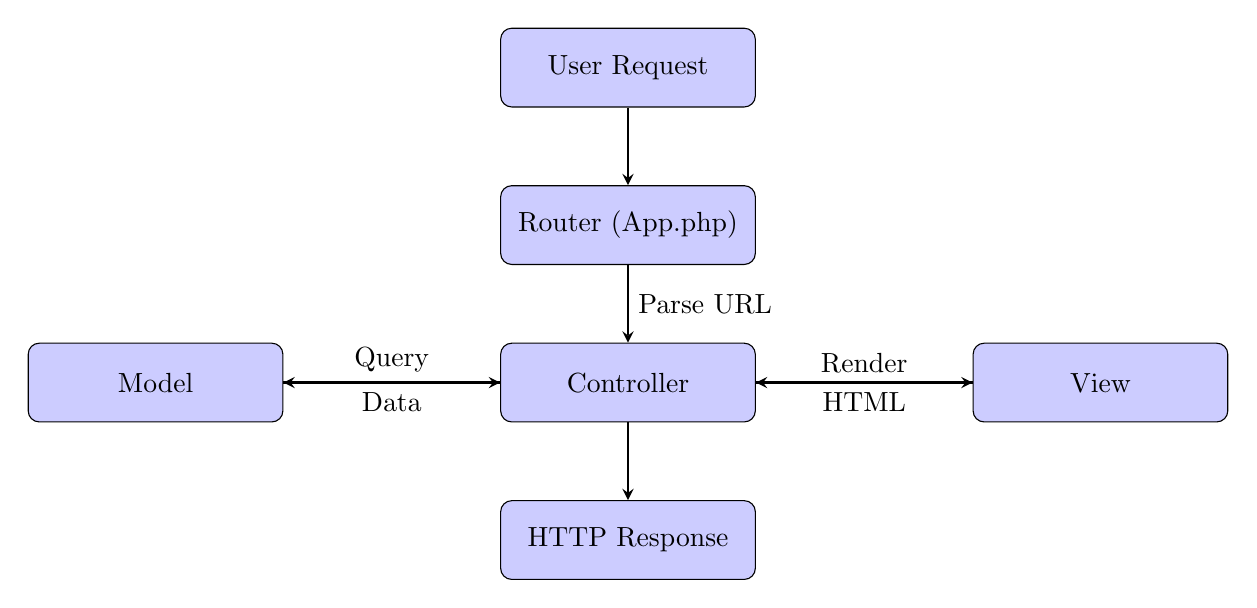
\begin{tikzpicture}[node distance=2cm, auto,
    box/.style={rectangle, draw, fill=blue!20, text width=3cm, text centered, rounded corners, minimum height=1cm},
    arrow/.style={->,>=stealth,thick}]

    \node[box] (user) {User Request};
    \node[box, below of=user] (router) {Router (App.php)};
    \node[box, below of=router] (controller) {Controller};
    \node[box, left of=controller, node distance=6cm] (model) {Model};
    \node[box, right of=controller, node distance=6cm] (view) {View};
    \node[box, below of=controller] (response) {HTTP Response};

    \draw[arrow] (user) -- (router);
    \draw[arrow] (router) -- node[right] {Parse URL} (controller);
    \draw[arrow] (controller) -- node[above] {Query} (model);
    \draw[arrow] (model) -- node[below] {Data} (controller);
    \draw[arrow] (controller) -- node[above] {Render} (view);
    \draw[arrow] (view) -- node[below] {HTML} (controller);
    \draw[arrow] (controller) -- (response);
\end{tikzpicture}
\caption{Luồng xử lý request trong mô hình MVC}
\label{fig:mvc-flow}
\end{figure}

\subsubsection{Các thành phần Core}

\textbf{1. Router - App.php:}
\begin{itemize}
    \item Parse URL thành: \texttt{[controller, method, params]}
    \item Load controller tương ứng
    \item Gọi method với parameters
    \item Xử lý 404 nếu không tìm thấy
\end{itemize}

\textbf{2. Base Controller - Controller.php:}
\begin{itemize}
    \item \texttt{model(\$name)}: Load model động
    \item \texttt{view(\$view, \$data)}: Render view với data
    \item \texttt{redirect(\$path)}: Chuyển hướng trang
    \item \texttt{isPost()}, \texttt{isGet()}: Kiểm tra HTTP method
\end{itemize}

\textbf{3. Database Wrapper - DB.php:}
\begin{itemize}
    \item PDO connection singleton
    \item \texttt{query(\$sql, \$params)}: Execute với prepared statements
    \item \texttt{single()}, \texttt{all()}: Fetch results
    \item Transaction support
\end{itemize}


% ------------------------------------------
\subsection{Cấu trúc thư mục}

Dự án được tổ chức theo cấu trúc MVC rõ ràng:

\begin{verbatim}
BTL_Fahasa/
|-- app/                      # Application code
|   |-- config/               # Configuration files
|   |-- controllers/          # Controller classes
|   |-- core/                 # Core framework files
|   |-- models/               # Model classes
|   +-- views/                # View templates
|-- public/                   # Public assets
|   |-- index.php             # Entry point
|   |-- css/                  # Stylesheets
|   |-- js/                   # JavaScript files
|   +-- images/               # Images
+-- db/                       # Database files
\end{verbatim}


% ------------------------------------------
\subsection{Tính năng hệ thống}

\subsubsection{Khách (Guest)}

Người dùng chưa đăng nhập có thể:
\begin{itemize}
    \item Truy cập trang chủ và xem sản phẩm nổi bật
    \item Duyệt danh sách sản phẩm theo danh mục
    \item Xem chi tiết sản phẩm
    \item Tìm kiếm sản phẩm
    \item Đọc tin tức và bài viết
    \item Xem trang giới thiệu, hỏi đáp, liên hệ
    \item Đăng ký tài khoản mới
    \item Đăng nhập vào hệ thống
\end{itemize}

\subsubsection{Thành viên (Customer)}

Sau khi đăng nhập, thành viên có thêm các quyền:
\begin{itemize}
    \item Thêm sản phẩm vào giỏ hàng
    \item Quản lý giỏ hàng (tăng/giảm số lượng, xóa)
    \item Xem và chỉnh sửa thông tin cá nhân
    \item Xem lịch sử đơn hàng
    \item Quản lý danh sách sản phẩm yêu thích
    \item Nhận thông báo về đơn hàng
    \item Đăng xuất khỏi hệ thống
\end{itemize}

\subsubsection{Quản trị viên (Admin)}

\textit{Lưu ý: Tính năng admin chưa được triển khai đầy đủ trong phiên bản hiện tại.}

Các tính năng dự kiến:
\begin{itemize}
    \item Quản lý danh sách người dùng
    \item Thêm/sửa/xóa sản phẩm
    \item Quản lý danh mục sản phẩm
    \item Xử lý đơn hàng
    \item Quản lý nội dung tin tức
    \item Xem thống kê và báo cáo
\end{itemize}

% ------------------------------------------
\subsection{Luồng hoạt động (Flowcharts)}

\textbf{Luồng đăng nhập:}
\begin{enumerate}
    \item Người dùng truy cập trang đăng nhập
    \item Nhập username và password
    \item Hệ thống kiểm tra thông tin
    \item Nếu đúng: Tạo session, redirect về trang chủ
    \item Nếu sai: Hiển thị thông báo lỗi
\end{enumerate}

\textbf{Luồng mua hàng:}
\begin{enumerate}
    \item Khách hàng duyệt sản phẩm
    \item Click "Thêm vào giỏ" trên sản phẩm mong muốn
    \item Kiểm tra đăng nhập - nếu chưa, yêu cầu đăng nhập
    \item Sản phẩm được thêm vào giỏ hàng (Session)
    \item Khách hàng có thể tiếp tục mua hoặc checkout
    \item Xem giỏ hàng, điều chỉnh số lượng
    \item Tiến hành thanh toán
    \item Xác nhận đơn hàng
\end{enumerate}
